\documentclass[12pt]{article}
\usepackage[a4paper]{geometry}
\pdfoutput=1
% \usepackage{preiclr,times}
\usepackage{iclr2017_conference,times}
\usepackage[english]{babel}
\usepackage{hyperref}
\usepackage{url}
\usepackage{amssymb}
\usepackage{amsfonts}
\usepackage{amsmath}
\usepackage{graphicx}
\graphicspath{{images/}}
\usepackage{cleveref}
\newtheorem{theorem}{Theorem}
\newtheorem{lemma}{Lemma}
\crefname{lemma}{Lemma}{Lemmas}
\usepackage{ccicons}
\usepackage{caption}

\iclrfinalcopy


\begin{document}
\begin{titlepage}
	\begin{center}
		
\includegraphics[width=0.6\textwidth]{UnivAQ-logo}\\[1cm]
		{\large University of L'Aquila}\\[0.5cm]
		{\large Department of Information Engineering, Computer Science and Mathematics}\\[0.5cm]
		\rule{\linewidth}{0.5mm} \\[0.4cm]
		{\huge \bfseries Hyper Heursitic Cryptography\\
			with\\
			Mixed Adversarial Nets \\[0.4cm] }
		\rule{\linewidth}{0.5mm} \\[1.5cm]
		\noindent
		\begin{minipage}{0.4\textwidth}
			\begin{flushleft}
				\large
				\emph{Author :}\\
				Aly \textsc{Shmahell}
			\end{flushleft}
		\end{minipage}%
		\begin{minipage}{0.4\textwidth}
			\begin{flushleft}
				\large
				\emph{Supervisor :} \\
				Prof.~Giovanni \textsc{De Gasperis}\\
			\end{flushleft}
		\end{minipage}
		\vfill
		\today
	\end{center}
\end{titlepage}
\begin{titlepage}
		\begin{center}
			
\includegraphics[angle=-90]{by-nc-sa}
		\end{center}
			\begin{center}
				This work is licensed under a
			\end{center}
			\begin{center}
				 \href{http://creativecommons.org/licenses/by-nc-sa/4.0/}{Creative Commons Attribution-NonCommercial-ShareAlike 4.0 International License.}
			\end{center}
		
\end{titlepage}
\begin{abstract}
Abstract
\end{abstract}
\newpage
\section{\textbf{Introduction}}\label{sec:introduction}
\subsection{\textbf{Xavier Initialization} \cite{DBLP:journals/jmlr/GlorotB10}}
When we talk about initialization, we mean the initial value which should be given to a certain neuron, this initial value is important for the neuron and for the network in general.\\
\begin{lemma}\label{lemma1}
Suppose our net uses the hyperbolic tangent activation function for its neurons:\\
\begin{center}
	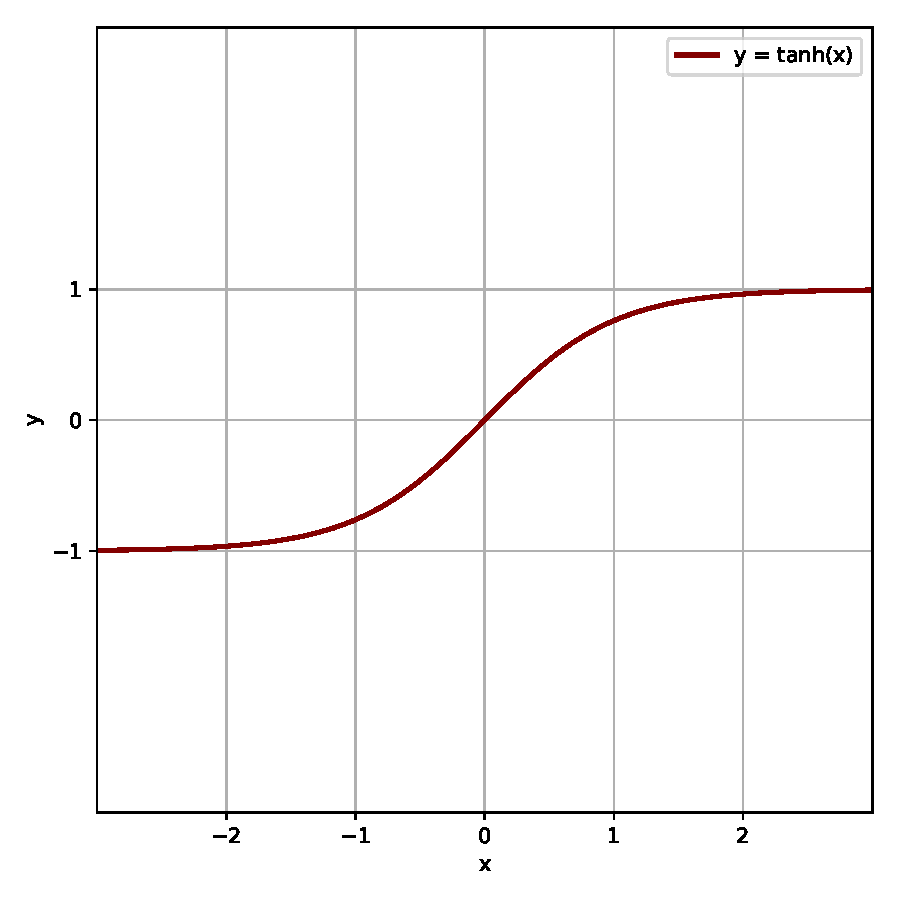
\includegraphics[width=0.6\textwidth]{tanh}\\[1cm]
\end{center}
\begin{itemize}
	\item If the weights start too small, then the signal shrinks as it passes through each layer until it vanishes, then as it passes deeper in the network with its small values, the layers it enter will become linear, because the output of the hyperbolic tangent is linear with small input values, this means the deeper layers of the net will loose non-linearity.
	\item If the weights start too large, then the signal grows as it passes through each layer until it becomes too large, then as it passes deeper in the network with its large values, the layers it enter will become saturated, as the output of the hyperbolic tangent is flat with large input values, and this flatness will cause the gradient to become zero, and we will get the vanishing gradient problem.
\end{itemize}
\end{lemma}
\begin{lemma}\label{lemma2}
Having a pre-defined net graph: for each neuron we know the number of inputs and the number of outputs, therefor we can calculate a reasonable weight for the neuron in question based on a normal distribution of a zero mean and a 1/n variance.
\end{lemma}
\begin{lemma}\label{lemma3}
To achieve initialization while avoiding the two obstacles in \cref{lemma1}, we want the variance to remain the same with each passing layer.	
\end{lemma}
\newpage
Suppose we have an input X from a previous layer with n components and a linear neuron with random weights W in the current layer that spits out the same output Y to some neurons in the next layer.
\begin{center}
	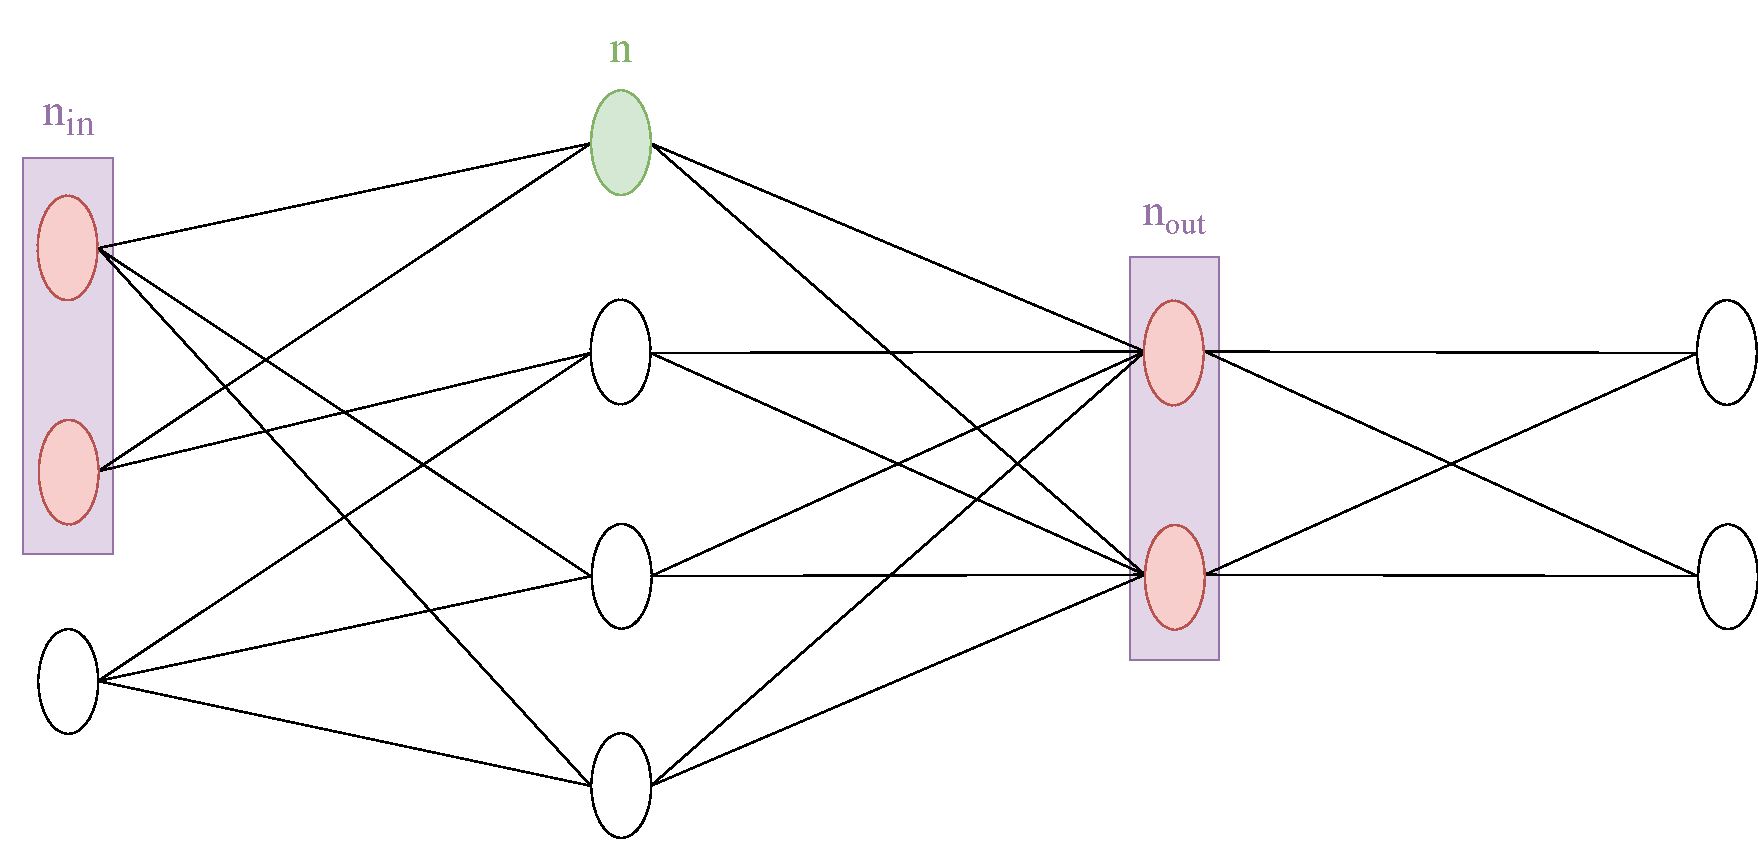
\includegraphics[width=0.6\textwidth]{xavier_illustration}
\end{center}
The output of the neuron will have the following equation:
\begin{center}
	\begin{equation}
		Y = W_1X_1 + W_2X_2 + ... + W_n X_n \label{eq:1}
	\end{equation}
\end{center}
To calculate the variance of each component:
\begin{center}
	\begin{equation}
		Var(W_iX_i) = E[X_i]^2 Var(W_i) + E[W_i]^2 Var(X_i) + Var(W_i)Var(X_i) \label{eq:2}
	\end{equation}
\end{center}
Since our inputs and weights come from a normal distribution of zero mean (from \cref{lemma2}):
\begin{center}
	\begin{equation}
		E[X_i]^2 Var(W_i) + E[W_i]^2 Var(X_i) = 0 \implies
		Var(W_iX_i) = Var(W_i)Var(X_i) \label{eq:3}
	\end{equation}
\end{center}
Since the neurons in the same previous layer are all independent, we assume that both $ X_i $ and $ W_i $  are independent and also identically distributed:
\begin{center}
	\begin{equation}
	 Var(Y) = Var(W_1X_1 + W_2X_2 + ... + W_n X_n) = nVar(W_i)Var(X_i) \label{eq:4}
	\end{equation}
\end{center}
In the last equation, we have the variance of the inputs, the variance of the output and the variance of the weights, now we can calculate the variance of the weights from ~\cref{lemma3}:
\begin{center}
	\begin{equation}
	 Var(Y) = Var(X_i) \implies Var(W_i) = \frac{1}{n_{in}} \implies Var(W_i) * n_{in} = 1  \label{eq:5}
	\end{equation}
\end{center}
Now if we go through the same derivation for back-propagation, we get:
\begin{center}
	\begin{equation}
	Var(W_i) = \frac{1}{n_{out}} \implies Var(W_i) * n_{out} = 1 \label{eq:6}
	\end{equation}
\end{center}
To keep the variance of the input gradient \& the output gradient the same, we combine
\eqref{eq:5} \& \eqref{eq:6} and we get:
\begin{center}
	\begin{equation}
	(n_{out} + n_{in}) * Var(W_i) = 2 \implies Var(W_i) = \frac{2}{n_{in} + n_{out}} \label{eq:7}
	\end{equation}
\end{center}
\newpage
\subsection{\textbf{1D Convolution on Batch 1D Data with multi-D Filters}}
	\begin{figure}[!htbp]
		\begin{center}
			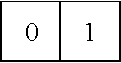
\includegraphics[width=0.1\textwidth]{input1}
			\caption{First Input String}
		\end{center}
	\end{figure}	
\begin{figure}[!htbp]
\begin{center}
	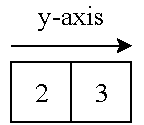
\includegraphics[width=0.1\textwidth]{input2}
	\caption{Second Input String}
\end{center}
\end{figure}
\begin{figure}[!htbp]
\begin{center}
	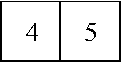
\includegraphics[width=0.1\textwidth]{input3}
	\caption{Third Input String}
\end{center}
\end{figure}
\begin{figure}[!htbp]
\begin{center}
	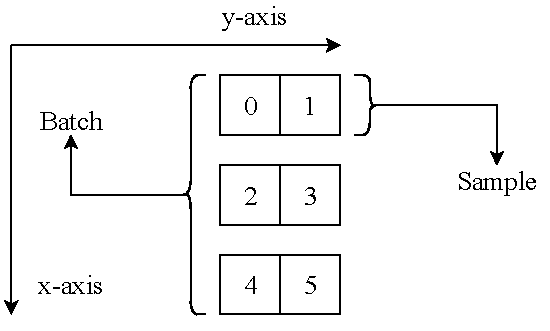
\includegraphics[width=0.1\textwidth]{input_final}
	\caption{Input Batch}
\end{center}
\end{figure}
\begin{figure}[!htbp]
\begin{center}
	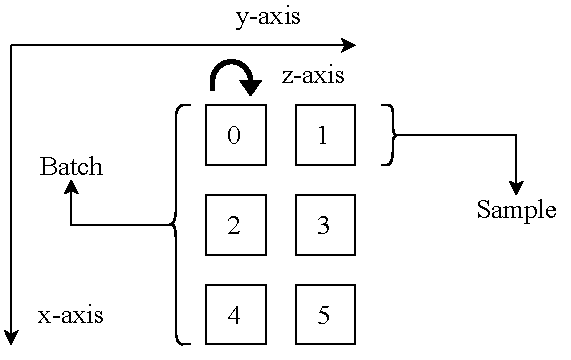
\includegraphics[width=0.1\textwidth]{input_reshaped}
	\caption{Reshaped Input Batch}
\end{center}
\end{figure}
\begin{figure}[!htbp]
\begin{center}
	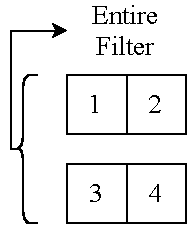
\includegraphics[width=0.1\textwidth]{filter1}
	\caption{First Filter}
\end{center}
\end{figure}
\newpage
\begin{figure}[!htbp]
\begin{center}
	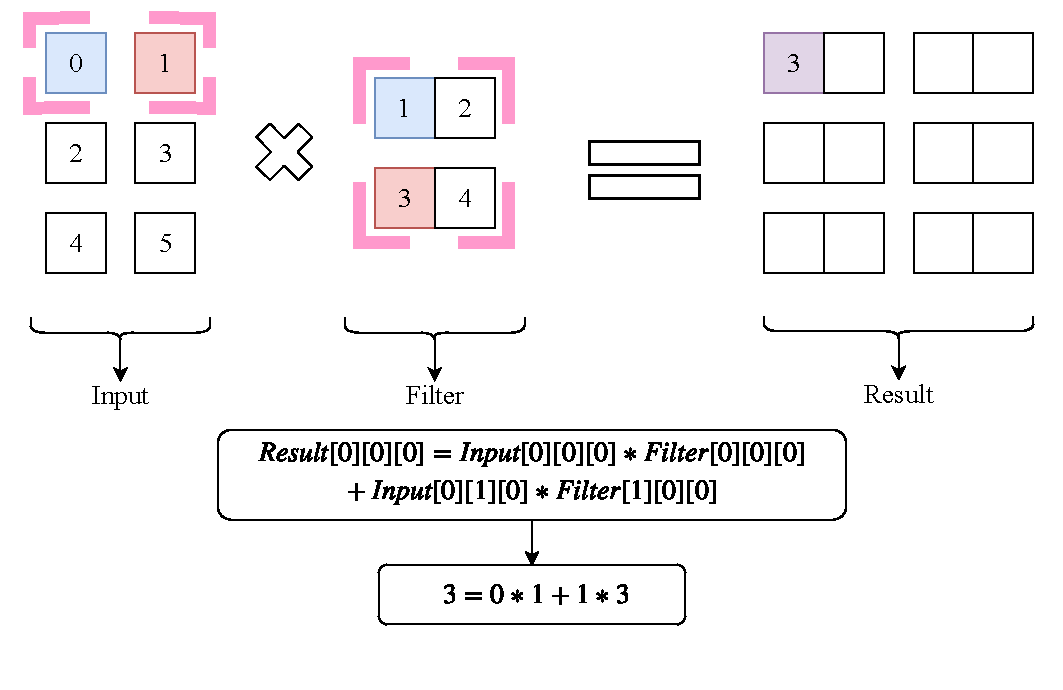
\includegraphics[width=\textwidth]{firstConvSample_step1}
	\caption{Applying the filter to the first sample in the input batch - }
\end{center}
\end{figure}
\begin{figure}[!htbp]
\begin{center}
	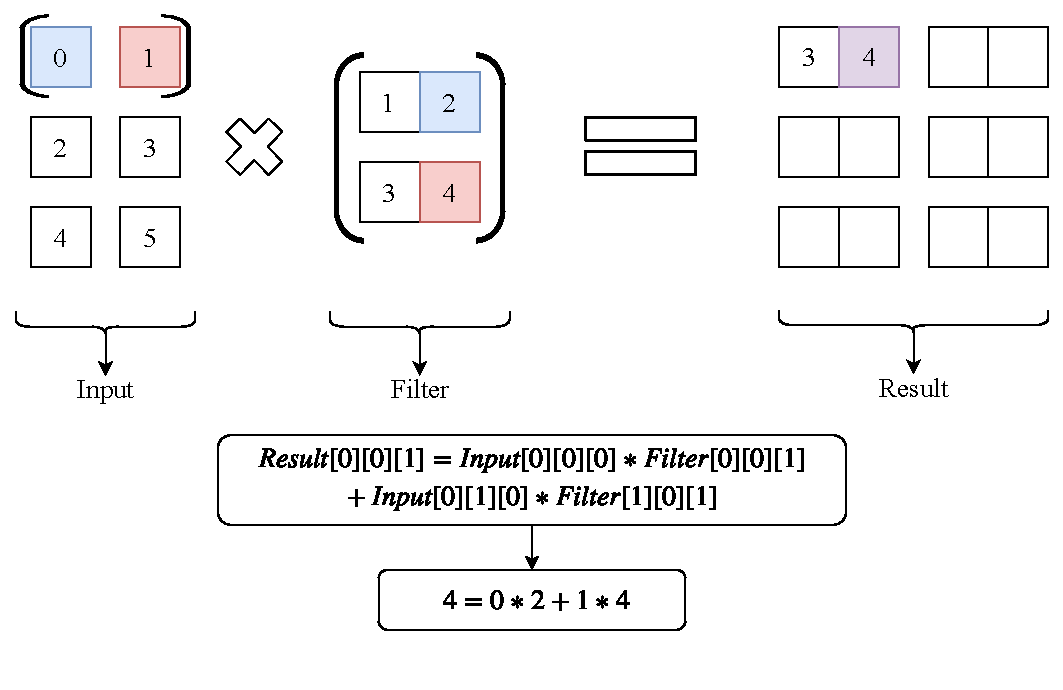
\includegraphics[width=\textwidth]{firstConvSample_step2}
\end{center}
\end{figure}
\begin{figure}[!htbp]
\begin{center}
	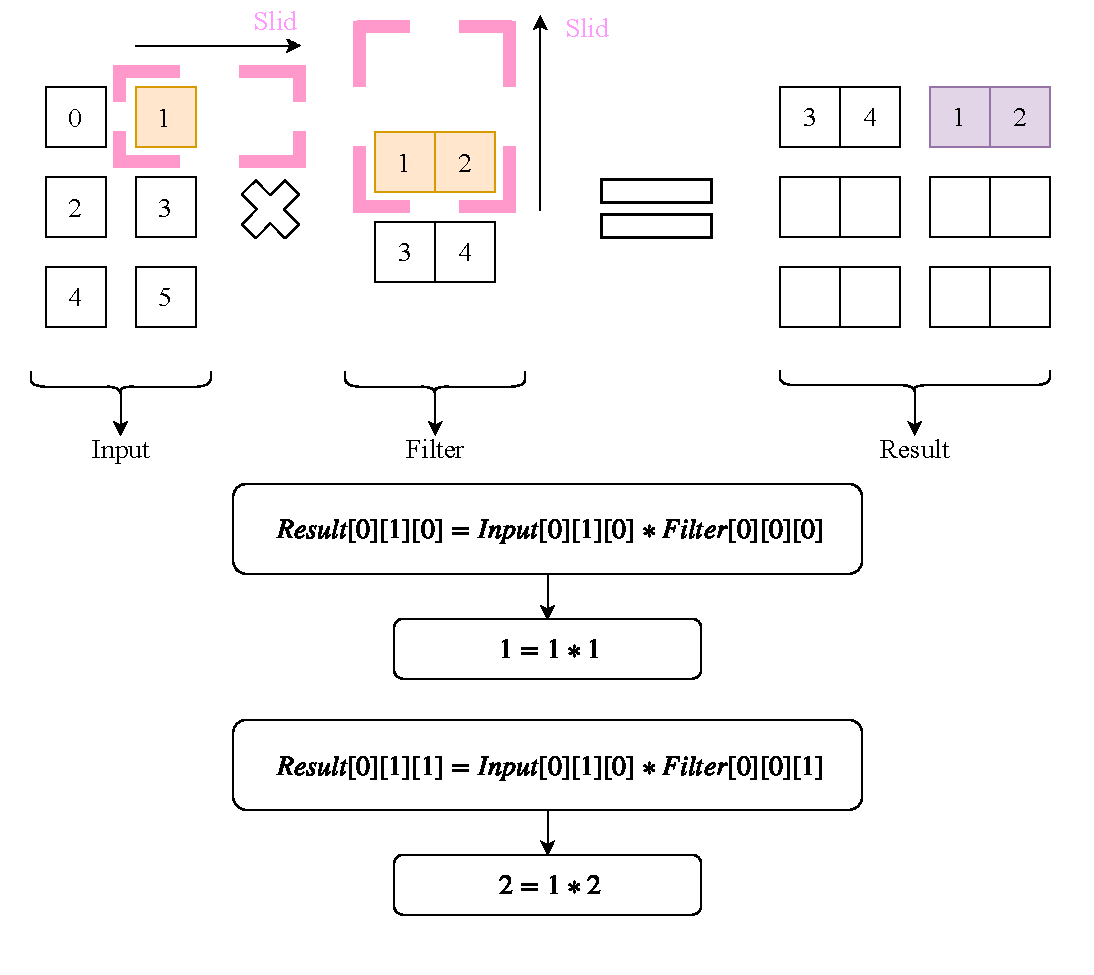
\includegraphics[width=\textwidth]{firstConvSample_step3}
\end{center}
\end{figure}
\begin{figure}[!htbp]
\begin{center}
	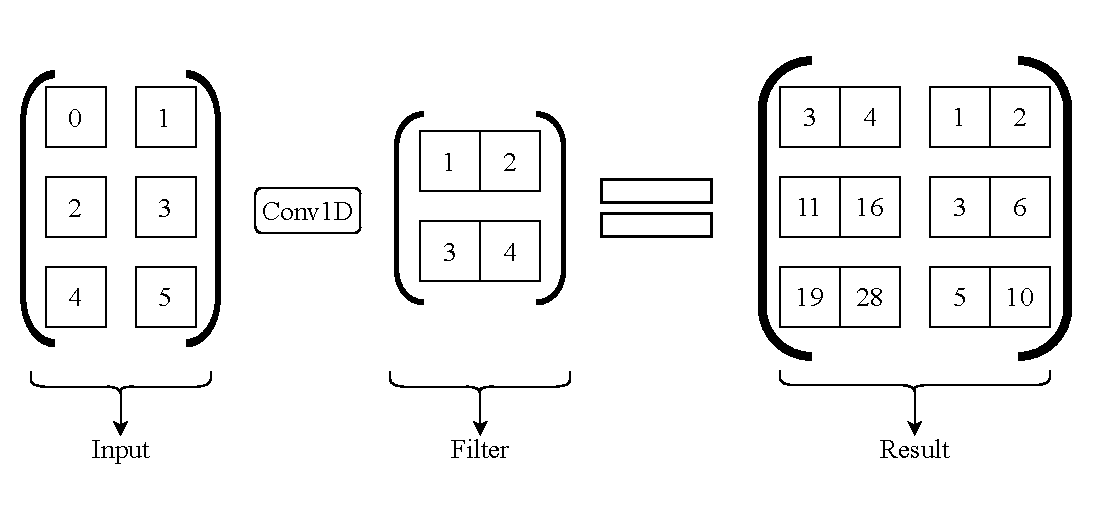
\includegraphics[width=\textwidth]{firstConvSample_final}
\end{center}
\end{figure}
\begin{figure}[!htbp]
\newpage
\begin{center}
	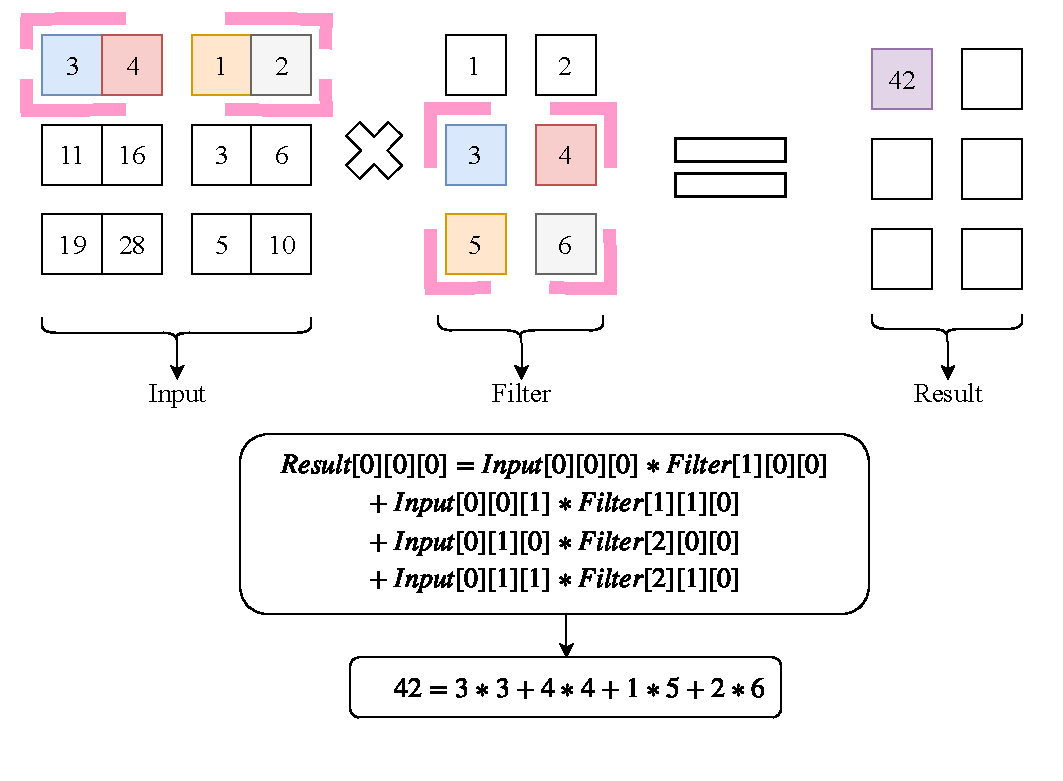
\includegraphics[width=\textwidth]{secondConvSample_step1}
\end{center}
\end{figure}
\begin{figure}[!htbp]
\begin{center}
	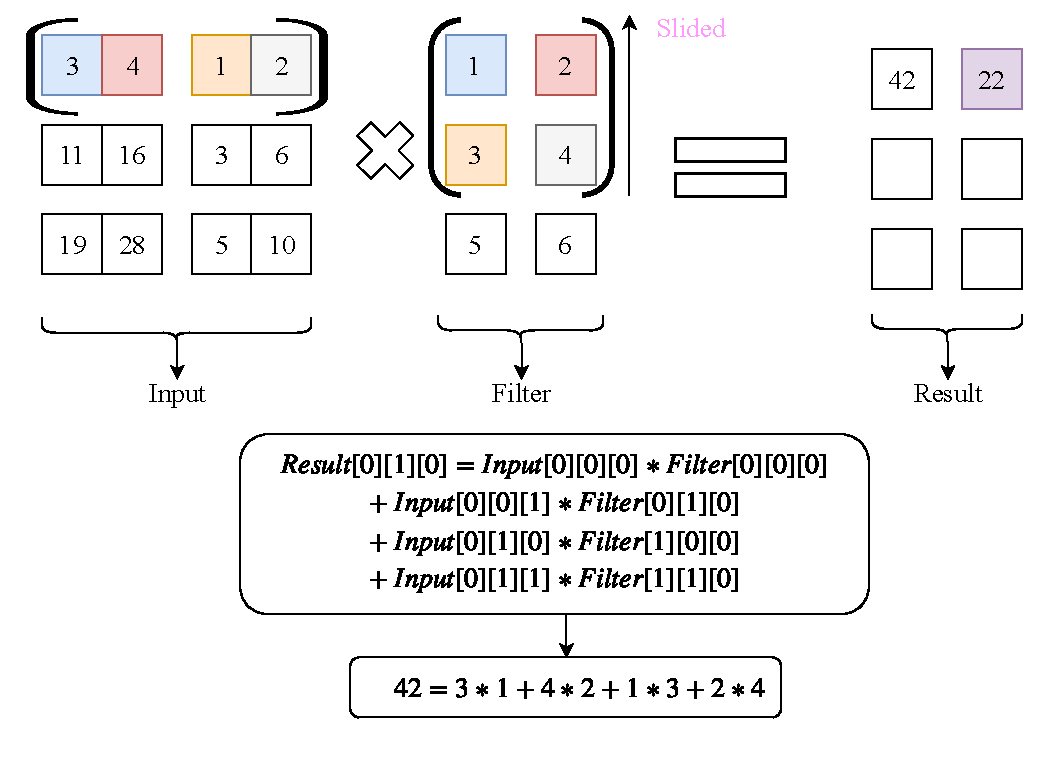
\includegraphics[width=\textwidth]{secondConvSample_step2}
\end{center}
\end{figure}
\begin{figure}[!htbp]
\begin{center}
	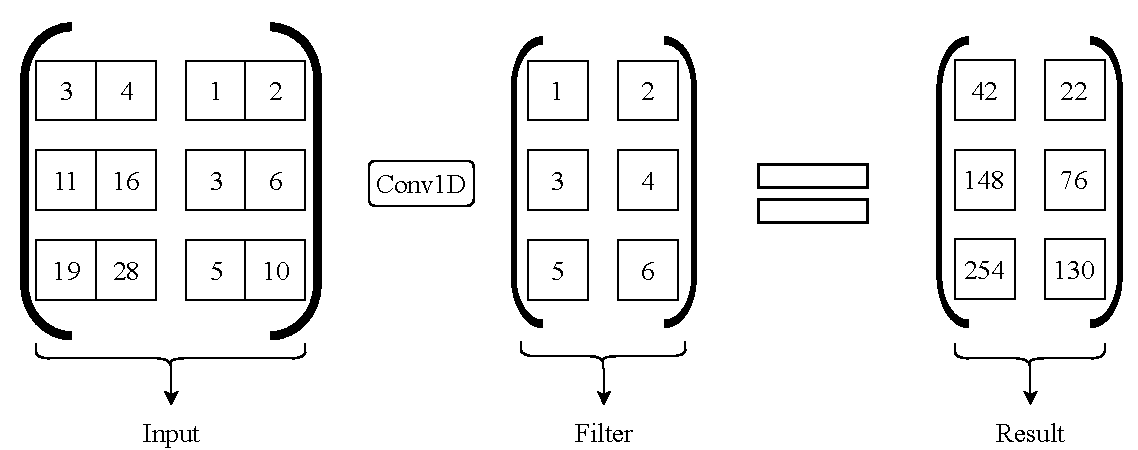
\includegraphics[width=\textwidth]{secondConvSample_final}
\end{center}
\end{figure}
\newpage
\section{\textbf{Design}}\label{sec:design}
	
\newpage
\section{\textbf{Implementation}}\label{sec:implementation}
\newpage
\section{\textbf{Conclusion}}\label{sec:conclusion}
\newpage

\medskip
\bibliographystyle{unsrt}
\bibliography{neurencoder}
\newpage

\appendix
\section*{\textbf{Appendix}}

\end{document}